\section{Multi-level Selective Deduplication}
\label{sect:arch}

\subsection{Snapshot Service Architecture}
%\subsection{Aliyun's VM Cloud and 
Our architecture is built on the Aliyun platform which provides the largest public VM cloud in China 
based on Xen~\cite{Xen2003}. A typical VM cluster in our cloud environment
consists of from hundreds to thousands of physical machines, each of which can
host tens of VMs. A few varieties of mainstream OS are supported.
%including several editions of Windows Server, major Linux distributions, and FreeBSD.
During the VM creation, a user chooses her flavor of OS distribution and the cloud system 
copies the corresponding pre-configured base VM image to her VM as the OS disk, 
and an empty data disk is created and mounted onto her VM as well. 
All these virtual disks are represented as virtual machine image files in our
underline runtime VM storage system. The runtime I/O between virtual machine and its virtual
disks is tunneled by the virtual device driver (called TapDisk at Xen). To avoid network latency and congestion, 
Aliyun's distributed file system carefully selects the location of primary replica of VM's 
image files such that they are located on the same physical machine of VM instance.
During snapshot backup, concurrent disk write is logged 
so that each snapshot can have a   consistent version.

Figure~\ref{fig:arch} shows the architecture view of snapshot service with selective deduplication
at each node. The  snapshot broker provides the functional interface for  snapshot backup, access, and deletion.
In accomplishing such a function, this broker accesses  the snapshot store managed by the underlying distributed file
system.  The inner VM  deduplication is conducted by the broker to access meta data in the snapshot data store
and we discuss this in details in Section~\ref{sect:innerVM}.
The inter-VM deduplication is conducted by the broker to access a  common data block set (CDS) across multiple VMs.
The CDS hash index is stored in the distributed memory cache. 

\begin{figure}[htbp]
  \centering
  %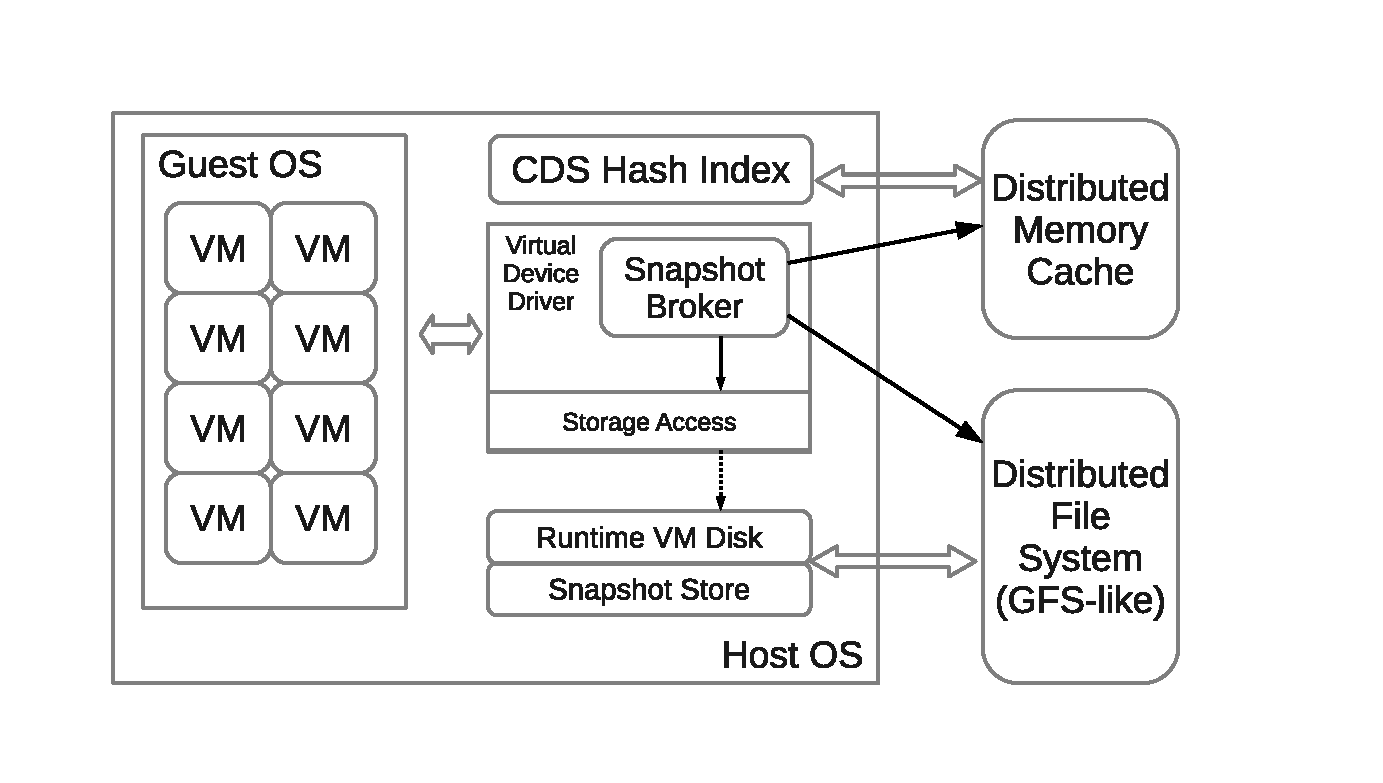
\epsfig{file=images/arch.eps, height=2in, width=2.66in}
  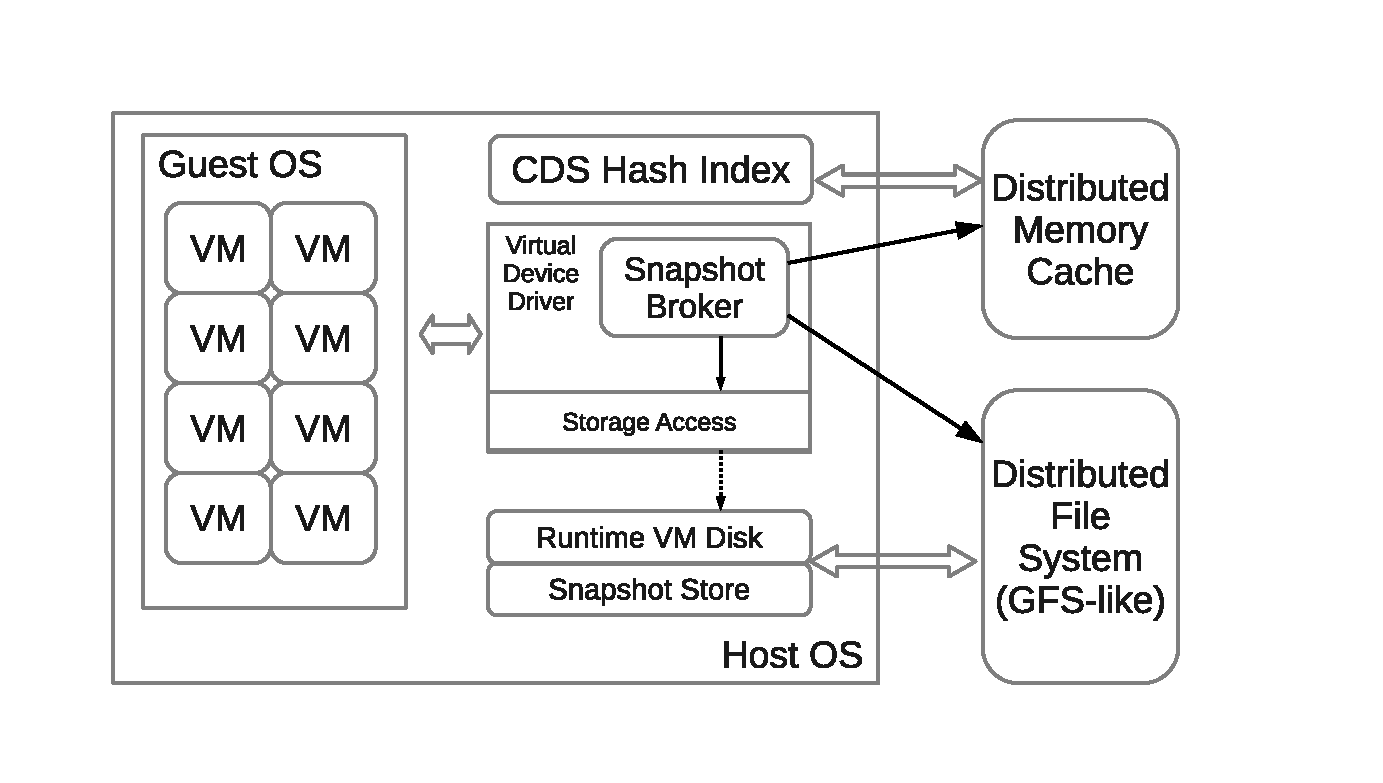
\epsfig{file=images/arch.eps, width=3.5in}
  \caption{Snapshot backup architecture of each node.}
  \label{fig:arch}
\end{figure}


The snapshot store  residing in the distributed file system
supports data access operations  such as \emph{get}, \emph{put} and \emph{delete}.
Other operations include data block traverse  and resource usage  report.
Snapshots are stored  in our distributed file system, just like regular virtual data files. 
A key  difference is that snapshot storage does not need to be
co-located within VM instances and  in fact they can even live in a different cluster to improve the 
data reliability. When a computing cluster is not available, we are still able to  restore users' VMs from another cluster which
contains snapshot backup and run these VMs. 
%to reduce the impact to our users.
%Get interface accepts a piece of data, write it to the underline data file, and return
%a reference to the caller. This reference then can be used in the put interface to
%retrive or delete the data, thus the caller of put interface must preserve the
%data reference for future use. 
%In addition to above standand data access operations, the snapshot service also supports
%\emph{scan} and \emph{quota} methods. Scan allows us to traverse all the data blocks of each VM
%in the snapshot store, and quota is used to acknowledge user how much space he
%has actually used.

With Aliyun's distributed file system support, the snapshot store operates 
\emph{append-only} files. Each virtual disk has its own data store, all data 
blocks after deduplication will be stored into that system.
Since all the underline data structures is append only,
upon a delete request, the corresponding data will only be marked rather than being deleted.
A compaction will take place when deleted data has accumulated to a certain threshold, thus 
reclaiming the disk space .




%The detail design and implementation of our distributed file system and various 
%storage subsystems would be too complicated to be intorduced here, and also beyond
%the scope of this paper. In the remaining section we will brief the model and interface of 
%our snapshot storage.

\subsection{Inner-VM Deduplication}
\label{sect:innerVM}

The first-level deduplication is logically localized within each VM.
%There are several reasons that we let each MS have  its own block store for localized duplication rather than sharing. 
%First, all data written to block store are already being processed by deduplication
%process, thus no sharing is necessary unless we want to perform additional deduplication
%inside the block store. Second, 
Such localization increases data independence between different  VM backups,
simplifies  snapshot  management and statistics collection during VM migration and termination,
and facilitates parallel execution of snapshot operations.
%Finally, this reduces the complexity of concurrent snapshot operations.

%\begin{figure}[htbp]
%  \centering
%  %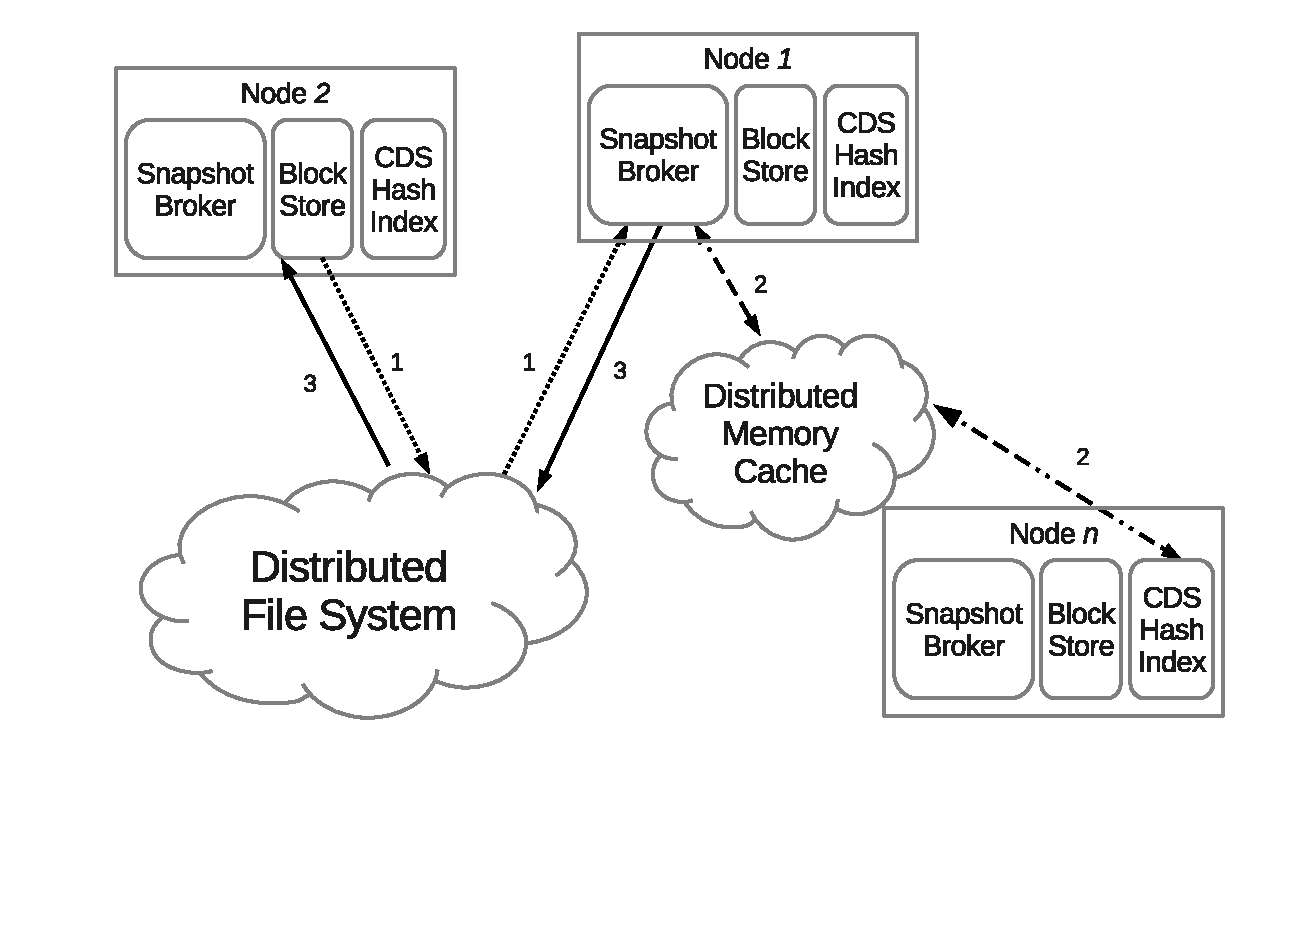
\epsfig{file=images/dedup_process.eps, height=2in, width=2.66in}
%  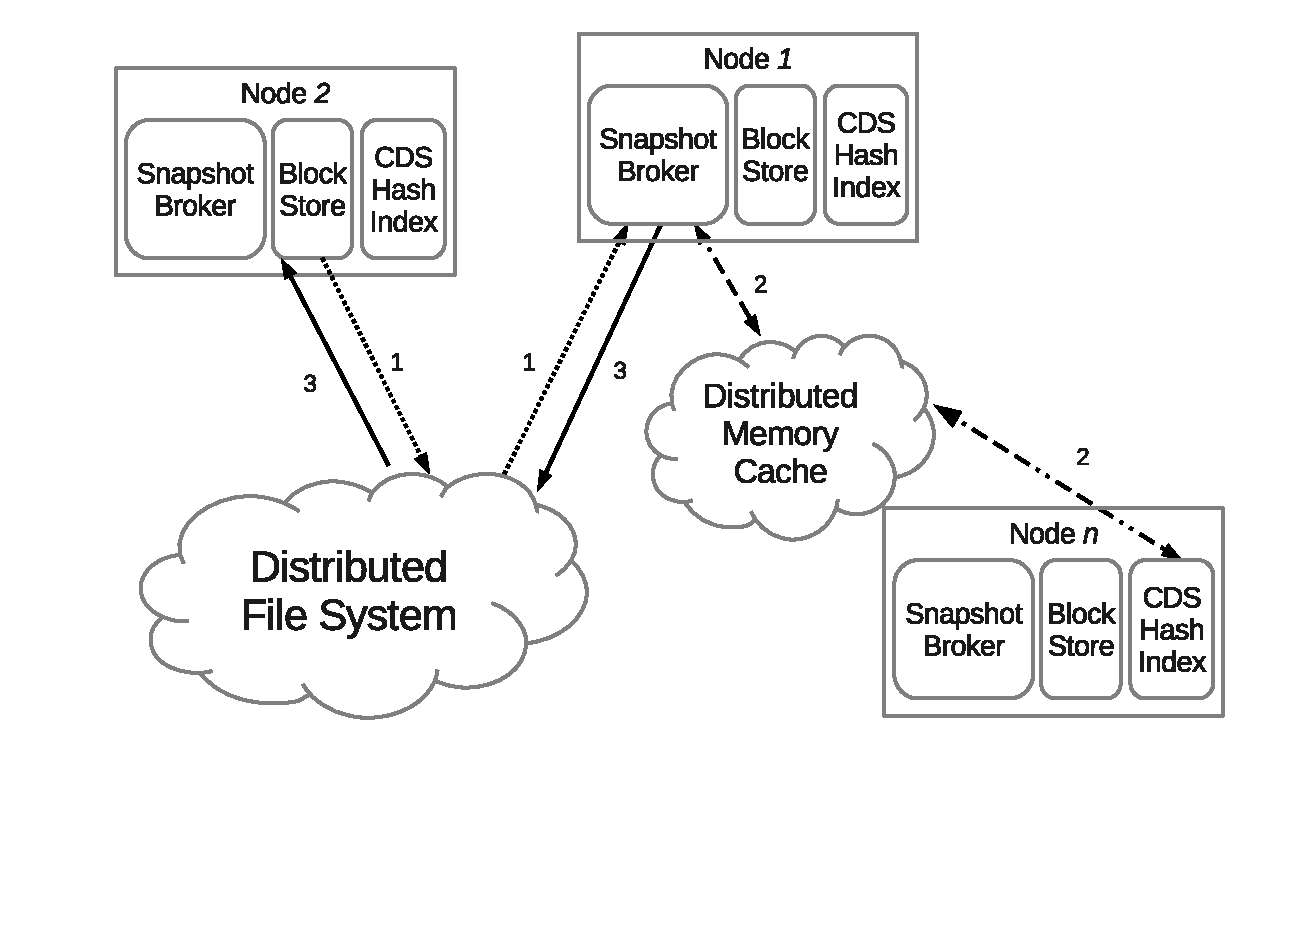
\epsfig{file=images/dedup_process.eps,  width=3.2in}
%  \caption{An example  of multi-level deduplication process.}
%  \label{fig:arch}
%\end{figure}
\begin{figure}[htbp]
  \centering
  %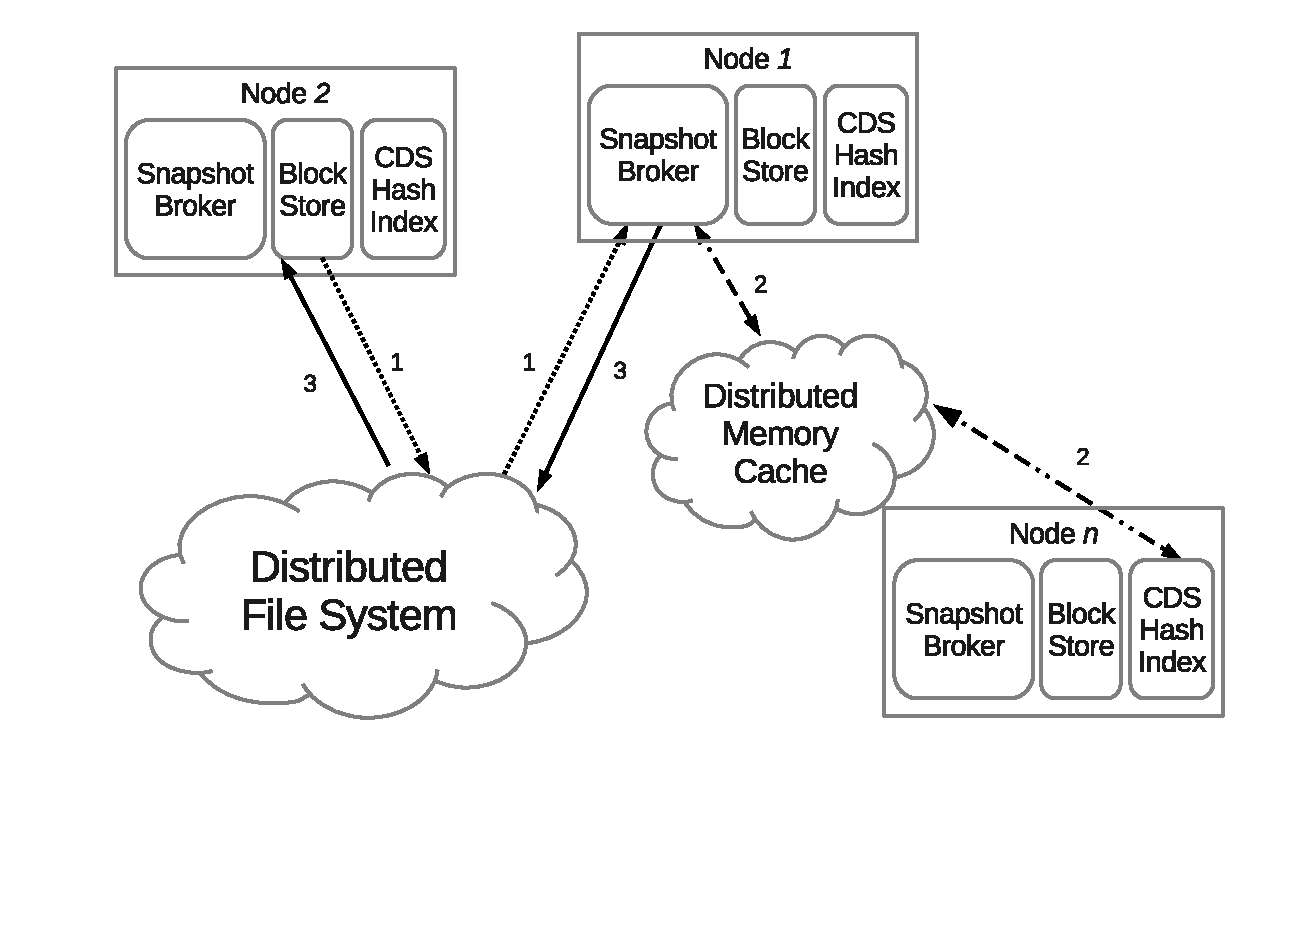
\epsfig{file=images/dedup_process.eps, height=2in, width=2.66in}
  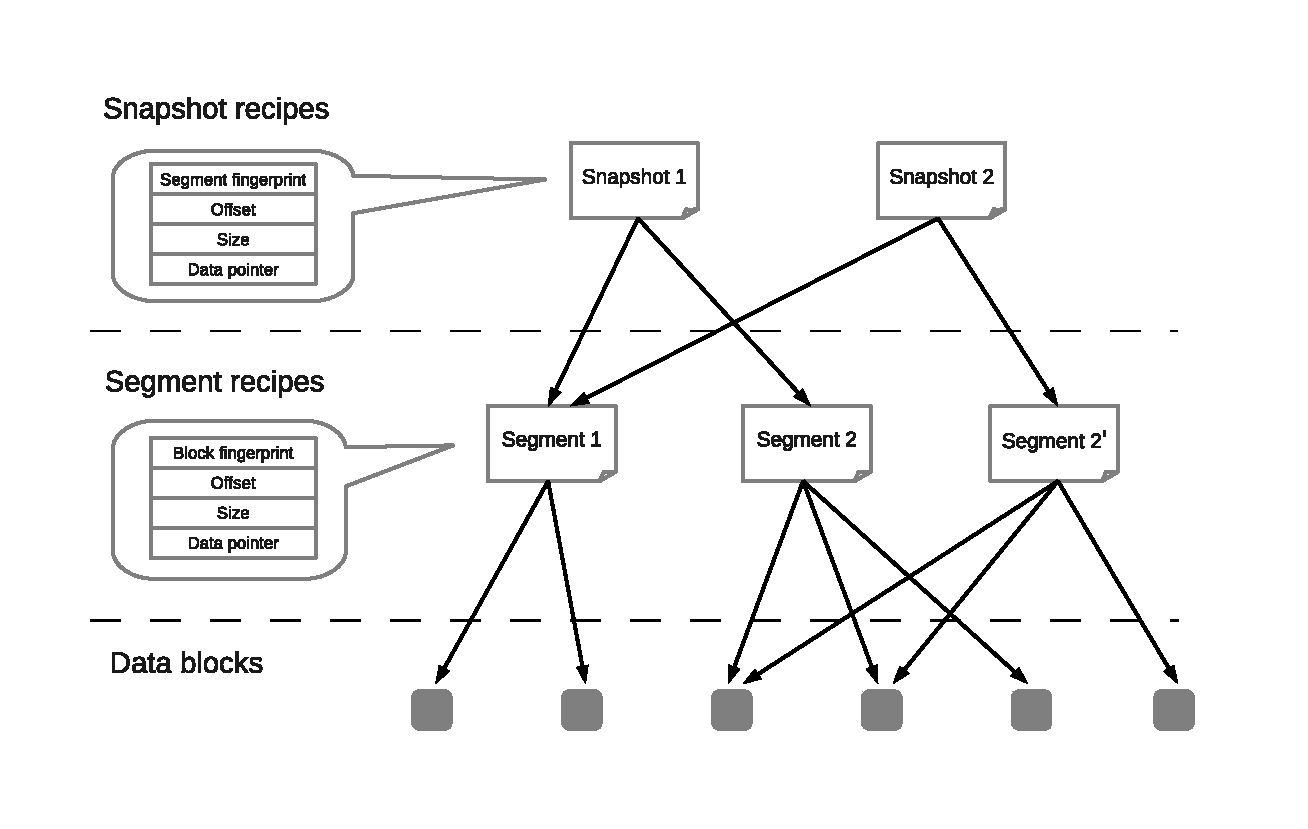
\epsfig{file=images/snapshot_representation.eps,  width=3.2in}
  \caption{An example  of snapshot representation.}
  \label{fig:snapshot}
\end{figure}

The inner VM deduplication contains two levels of duplicate detection efforts and the representation of
each snapshot is correspondingly designed as a two-level level index data structure in the form of a hierarchical
directed acyclic graph as shown in Figure~\ref{fig:snapshot}.
An image file is divided into a set of segments and each  segment contains hundreds of content blocks from the bottom level.
These blocks are of variable-size, partitioned using
the standard chunking technique~\cite{similar94}.  We use 4KB as the average block size. 
The segment metadata (called segment recipe) records its  content block hashes and  data reference. 
The snapshot-level recipe contains a set of  segment recipes and other meta data information.
\begin{itemize}
\item {\em Level 1 Segment modification  detection}.
If a segment is not changed, indicated by a dirty bit, its content blocks are not changed also. In this case,
 segment-level duplicate detection is more efficient than the block level. 

\item {\em Level 2  Block fingerprint comparison.}
If a segment is modified, content blocks of this segment are compared with 
the fingerprints of the existing content blocks within the same segment in
the previous version of this snapshot (called parent  snapshot). Partial duplication
within the segment can be detected and eliminated. 
\end{itemize}

We choose this two-level structure because in practice we observe that at each snapshot there are a large
number of content blocks which are not modified from one snapshot version to another.
Aggregating a large number of content blocks as one segment can significantly
reduce the space cost of snapshot meta data. 
%Namely the  snapshort metadata starts with
%the representation of segment-level meta data. Each segment receipe can be further represented by
%a set of content block receipes.

How can we choose the length of a segment?
Instead of using variables-sized segments, we take a simple approach
to let every segment being aligned to the page boundary of each virtual image file.
For Aliyun, each VM image file is represented as a virtual disk file format
(called \emph{vhd} at Xen) and we use a dirty bit to capture if a page (or segment) of a virtual snapshot file 
has been modified or not for segment-level deduplication.
%This is effective because  
%a vhd   file keeps the allocated inner blocks at the same positions until deletion,
%which means the locality of snapshot data is almost natively aligned. 
A dirty bit array is used to indicate which segments have been modified or not. 
Each page (segment) size in our implementation uses 2MB, which contains a large number of content blocks.
%Enforcing a boundary at every 2MB will 
%only break 0.2\% of total data blocks which is tiny.
% dirty bits array. This is because
%Inside the TapDisk driver, we maintain an array of \emph{dirty bits} to record the dirty area
%of runtime VM image file since the last snapshot, each bit represent a 2MB fix-sized
%data segment. During a snapshot operation, we only need to look at the dirty region
%rather than scan over the whold image file, which would be extremely slow.





%We let each virtual disk has its own block store rather than sharing for several reasons:
%first, all data written to block store are already being processed by deduplication
%process, thus no sharing is necessary unless we want to perform additional deduplication
%inside the block store. Second, such seperation will facilitate VM data stastics, 
%deletion and migration. Finally, this reduces the complexity of concurrent snapshot operations.

Once level-2 deduplication is activated for those segments that have been modified,
it requires memory to load  block fingerprints from the corresponding
parent snapshot's segment.
This scheme processes one segment at time and each segment of 2MB contains about 
500 content blocks on average given 4KB is the average block size.
That only takes a tiny amount of space to hold their fingerprints.
%Given  1-2 hours of window to backup snapshots and every VM has  on average about 40GB, there is enough
%time to search all segments sequentially~\cite{NOT-CLEAR-HERE}

\subsection{Cross-VM Deduplication with CDS}

The third-level of deduplication is to identify duplicated data blocks among multiple VMs through the index cache
of common data set (CDS).  CDS is the most popular content blocks 
among  recent snapshots across all VMs. 
Each index entry contains  the block fingerprint and a reference pointer to the location of its real content
in the snapshot content block store residing in the underlying distributed file system.
%The structure of CDS meta is not different from the segment recipe we discussed above, 
%except that it is partitioned into many small slices so that each node is easy to load its own slice. 

At the runtime, the CDS index resides in a distributed  memory lookup table  
implemented using Memcached~\cite{memcached} to leverage the aggregated memory in a cluster.
Th usage of memory at each machine is small and thus  this scheme  does not
lead to  a memory resource contention with the existing cloud services.
%For example, in our current implementation setting at Aliyun, we use up to  150MB memory per node during night backup
%including CDS and other metadata for all levels of deduplication. Most of memory resource (48GB per node 
%in our experiment) is used for existing  applications.
CDS raw data stored  in the distributed file system
has multiple copies in different machines for the purpose of fault tolerance and 
while providing high read  throughput.  
%The data of CDS is stored in a special block store in the distribued file system.

% which doesn't belong to any VM disk.

%CDS meta assignment is done statically, each slice of CDS meta has one primary and two backup nodes.
%During the system bootup, snapshot storage controller will read the assignment, 
%load its primary portion of CDS meta from distributed file system. Loading the backup portion
%of CDS is due upon a query arrives for it. Everyday the CDS assignment and CDS data will be checked
% for updates and reloaded if necessary.

%Behind the scene there is a offline map-reduce job, which will periodically scan the block stores
%in the entire cluster and perform a ``word counting''. High frequency blocks are then added to the CDS if its count 
% is greater than threshold, which is pre-defined by the system memory restrictions.
To control the size of searchable common data in this global setting, we focus on those items that 
are most popular based on the historical snapshot data and the popular analysis is conducted periodically to ensure 
meta data freshness to match the latest data access trend.
There are two advantages to exploit this.
First, a smaller CDS reduces overall resource requirement while covering  most of data blocks in snapshots.
Second a smaller CDS makes the fault tolerance management  easier because we can replicate  more copies
to mitigate the failure.


In Aliyun's VM cloud, each VM explicitly maintains  one OS disk, plus  one or more data disks.
During VM's creation, its OS disk is directly copied from user's chosen base image.
Given the separation of OS disks and data disks, we study  their characteristics separately.
We expect that the operating system and along with popular software installations  are not frequently
modified or deleted. 
%base image data as a hint.Through users may change configurations, install software, or write user data into OS disk,
%Thus most of content blocks for the OS related snapshots  shall keep unchanged.
%This is verified in  Section~\ref{sect:exper}.
We have sampled  the  popularity of common blocks in the OS and data disks from a dataset
containing over 1,000 VMs and each has 10 snapshots.

The left part of Figure \ref{fig:zipf-data} shows the duplicate count  for different data blocks sorted by their ranking in 
terms of the duplication count. $Y$ axis is the popularity of a data block in a log scale 
measured its duplicate count among snapshots. $X$ axis is the identification of data blocks in a log scale
sorted by their duplicate rank.  The rank number  1  is the block with the highest number of duplicates.
The curve exhibits that the popularity of common data blocks partially follows a  Zipf-like distribution.
The right part of Figure \ref{fig:zipf-data} shows the duplicate count  for OS disk snapshot blocks sorted by their ranking.
%$Y$ axis is the popularity of an OS block in a log scale 
%measured its duplicate count among snapshots. $X$ axis is the identification of OS blocks in a log scale
%sorted by their duplicate rank.  
For the top ranked blocks, there is a flat line in terms of duplicate counts. That
is because there are a large number of OS blocks which have appeared in all copies of such OS releases.


\begin{figure}[htbp]
\centering
%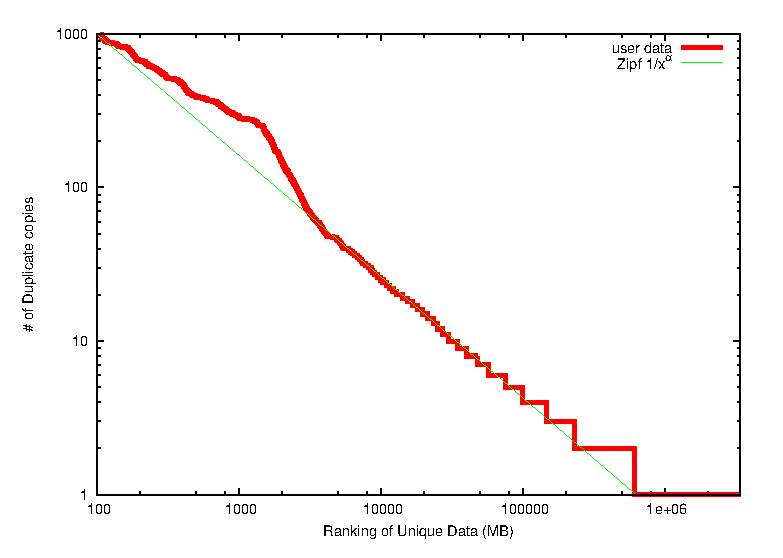
\epsfig{file=images/log-log.disk.eps, height=2in, width=2.66in}
%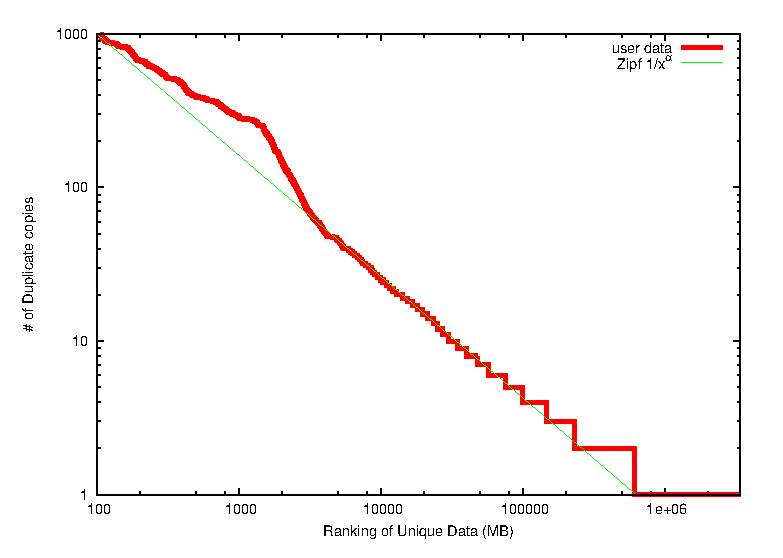
\epsfig{file=images/log-log.disk.eps, width=3in}

\begin{tabular}{cc}
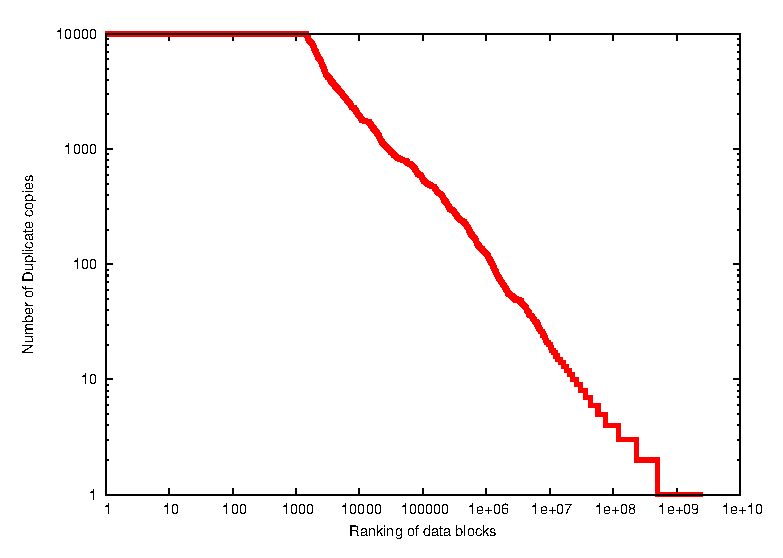
\epsfig{file=images/datadisk.count_rank.eps, width=1.5in} &
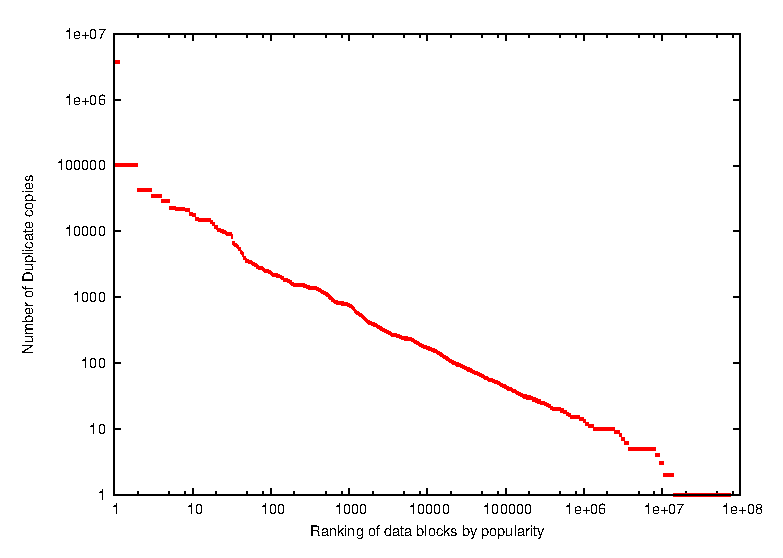
\epsfig{file=images/35vmos.count-rank.eps,width=1.5in}
\end{tabular}

\caption{Duplicate count  of common data blocks in a log scale on the left. The right is for common OS blocks.}
\label{fig:zipf-data}
\end{figure}

%\begin{figure}
%\centering
%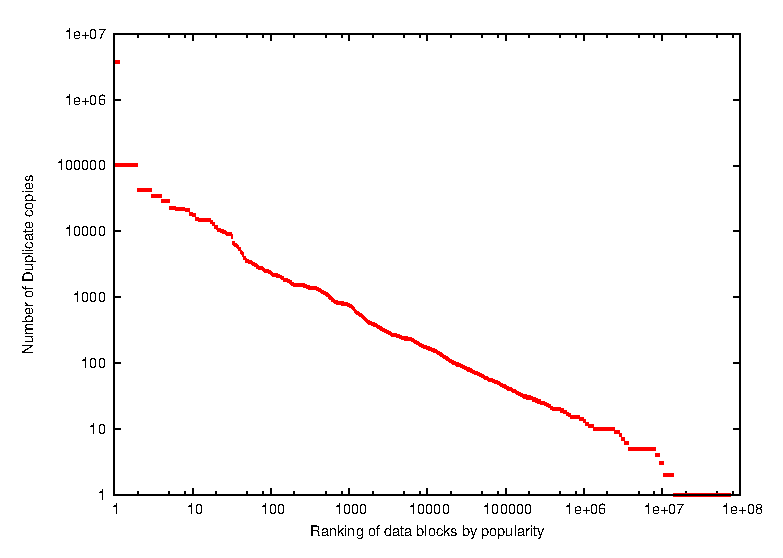
\epsfig{file=images/35vmos.count-rank.eps,width=3in}
%\caption{ Duplicate count of  common OS blocks in a log scale.}
%\label{fig:OSpopular}
%\end{figure}

As the number of VMs increases, the popularity of common blocks for data disks changes.
But this increase has a small impact on OS block popularity because 
there are a limited number of OS releases used by VMs. We let CDS cover the common OS blocks first and
our CDS selection strategy is designed as follows.
\begin{itemize}
\item First, most popular items from OS disks are selected.
Our experiment data shows that about 
100GB data from 7 most popular OS releases
can at least cover over 70\% of OS snapshots and the index of these 100GB OS blocks
only takes about total 1GB in the CDS index and then memory requirement per node for running the backup
on  a large cluster is tiny.
We expect that the OS CDS index may grow up to 2GB in order to cover large varieties  of commonly deployed
OS releases in practice.
\item Second, the degree of duplication is computed for snapshot blocks of data disks and
% and also snapshot 
%blocks of user data items stored in the OS disk (some users store data in their OS disks).
the  most popular items are selected. As discussed in Section~\ref{sect:exper}, 
that about 1\% of data blocks are selected based on their duplicate counts and these popular blocks
can cover about 38\% of data  blocks appeared in various snapshots after level 1 and level deduplication.  
The memory size per node used for CDS is within 150MB.
\end{itemize}
Thus in total the CDS index size per node takes less than 160MB in a large cluster bigger than 100 nodes based on
Aliyun's experiment data, covering over 53\% of blocks in OS and data disks after inner VM deduplication.
This memory usage is well below the limit required by Aliyun.


\subsection{Illustration  of multi-level deduplication process}


\comments{
\begin{figure*}
  \centering
  %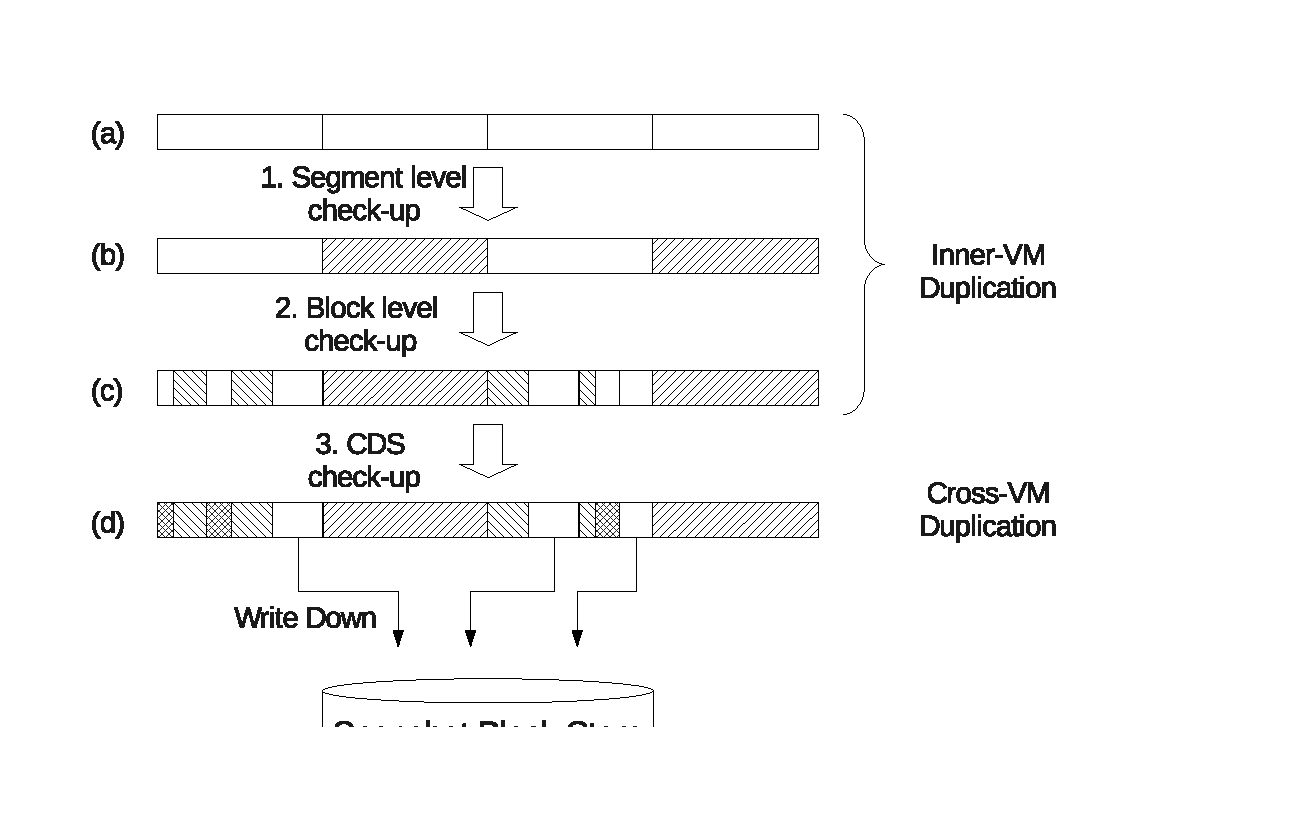
\epsfig{file=images/dedup_flow1.eps, height=2in, width=3.5in}
  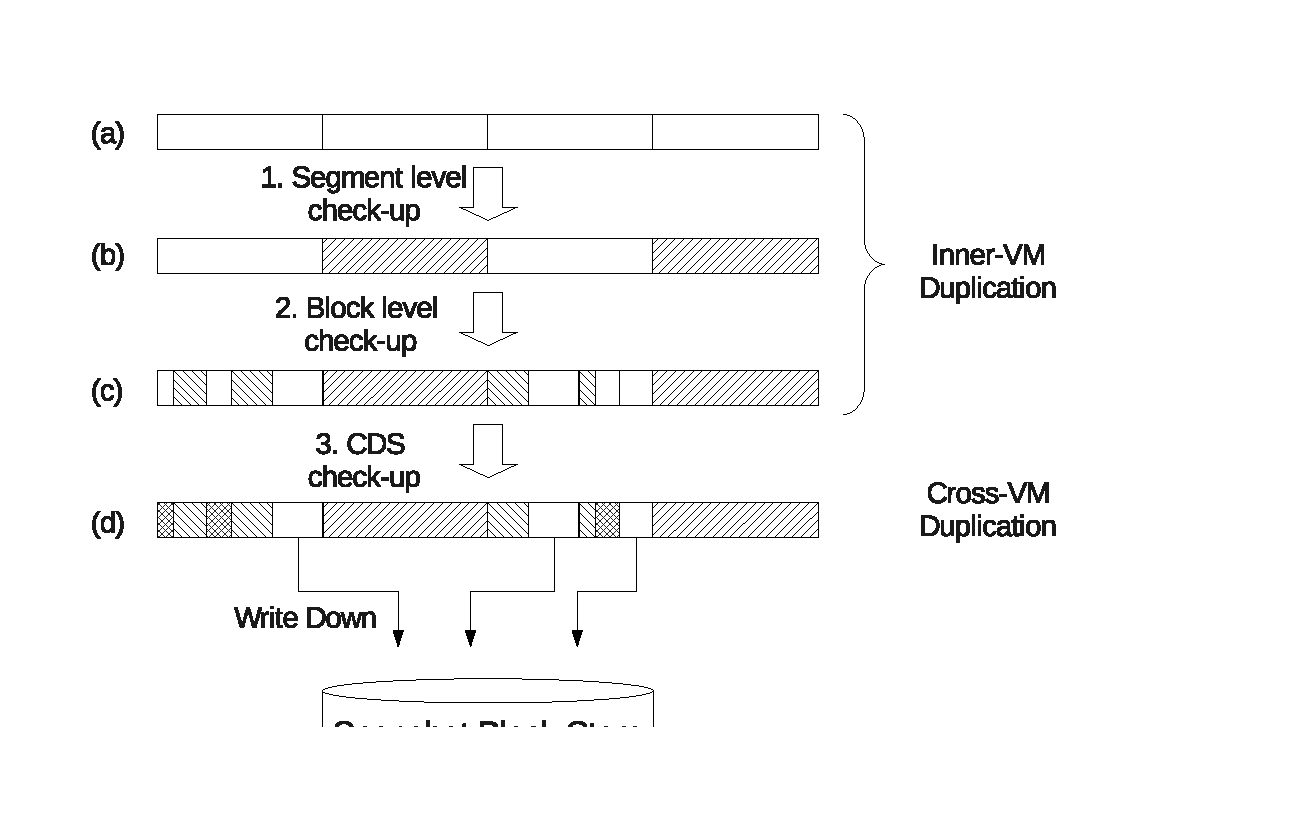
\epsfig{file=images/dedup_flow1.eps,  width=6in}
  \caption{Flow of deduplication.}
  \label{fig:tapdisk}
\end{figure*}
 

The 3-level deduplication process can be summarized as four steps:
\begin{list}{Dedup}{}
\item {Dirty bits: Copy the unchanged portion of snapshot recipe from parent snapshot, base on dirty bits.}
\item {Locality: Divide dirty segments into blocks, compare to the corresponding segment recipe at the same position of parent snapshot, if duplicate, copy the data reference into segment recipe.}
\item {CDS: Check if this data exist in the CDS, if yes, copy the returned data reference. Otherwise, write data block to block store, save the returned reference into segment recipe.}
\item {Save meta: write down the segment recipes and snapshot recipe when finish.}
\end{list}

}


%%Our deduplication process is divided into three levels, at each level, we eliminate the most of duplicate data with available knowledge, preventing them from going further because deduplication at deeper level is more expensive.
%
\begin{figure}
  \centering
  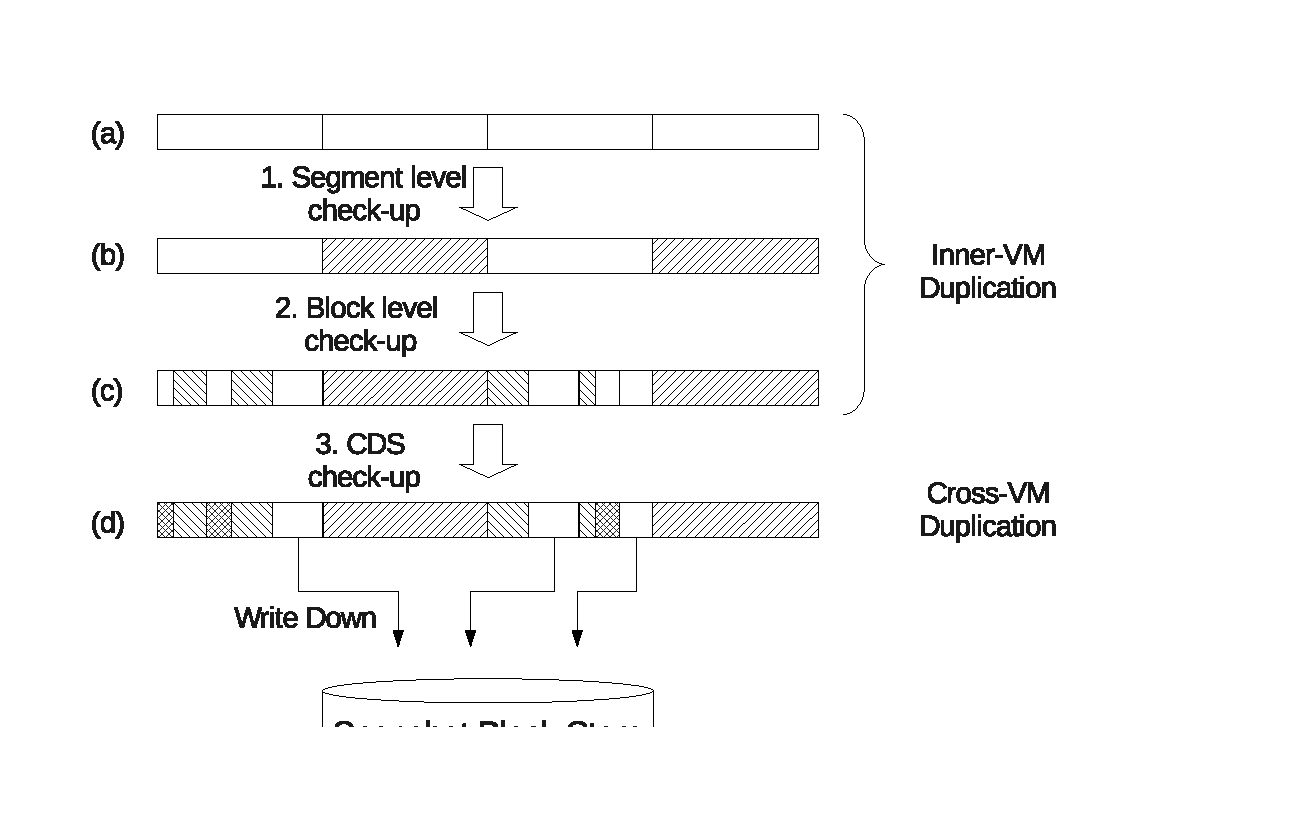
\epsfig{file=images/dedup_flow1.eps, height=2in, width=4in}
  \caption{Illustration of snapshot deduplication dataflow.}
  \label{fig:dedupflow}
\end{figure}

We illustrate the steps of 3-level deduplication in Figure~\ref{fig:dedupflow}, which can be summarized as 5 steps:
\begin{enumerate}
\item {\em Segment level checkup.}
As shown in Figure~\ref{fig:dedupflow} (a),
when  a snapshot of a plain virtual disk file is being created, we first check the dirty bitmap array of
this disk file  to see which segments are modified. If a segment is not modified since last snapshot, 
it's data pointer in the recipe of the  parent snapshot  can be directly copied into 
current snapshot recipe (shown as the shadow area in Figure~\ref{fig:dedupflow} (b)).

\item {\em Block level checkup.}
As shown in Figure~\ref{fig:dedupflow} (b),
for each dirty segment, we divide it into variable-sized blocks,
and compare their signatures with  the corresponding segment recipe in the previous snapshot version (called parent
snapshot). 
For any duplicated block, we copy the data pointer directly from the parent segment recipe. 
\item {\em CDS checkup.} For the remaining  content blocks whose duplicate status is unknown,
Figure~\ref{fig:dedupflow} (d)
shows  a further check to compare  them with  the cached signatures in the CDS by querying
the CDS hash index. If there is a match, the corresponding data pointer from the CDS index is
copied into the segment recipe. 
\item {\em Write new snapshot blocks :}
We continue the previous step and 
if a data block cannot be found in the CDS index, this block is considered to be a new block
and such a block is to be saved in the snapshot block store and  the returned reference  pointer is
saved in the  segment recipe.
\item {\em Save recipes.} Finally the  segment recipes are saved in the  snapshot block store also.
 After all segment recipes are saved, the snapshot recipe is complete and can be saved also.
\end{enumerate}

If there is no parent snapshot available, which happens when a VM creates its first snapshot, 
only CDS-based checkup will be conducted.
%This is important because most of the cross-VM duplication, such as OS related data and popular software data, is eliminated
%at this stage. Later snapshot will very likely find these data are not changed and simply copy the data pointers from parent snapshot.
